% Условная компиляция для самостоятельной работы
\ifdefined\mainfile
    % Если это часть основного файла, не добавляем начало и конец документа
\else
    \documentclass[12pt, a4paper]{report}
    \usepackage{/Users/vladbelousov/Desktop/Semestr_4-FP-NSU/Настройка/library}
    \usepackage[utf8]{inputenc} % Подключение поддержки UTF-8
    \begin{document}
\fi

%%-------------------------------%%

\[ U= -\frac{\alpha}{r }  \quad  \alpha= G M m - \text{задача Кеплера}   \] 

\( M  \)  - масса Солнца, планеты; \( m  \) - масса движущегося тела.

\[ U_{\text{эф} } = -\frac{\alpha}{r }  + \frac{ M ^2 }{2m r ^2 }   \] 

\[ r(\varphi ) = \frac{p}{1+ e \cos (\varphi - \varphi_0 )}  \] 

\begin{center}
    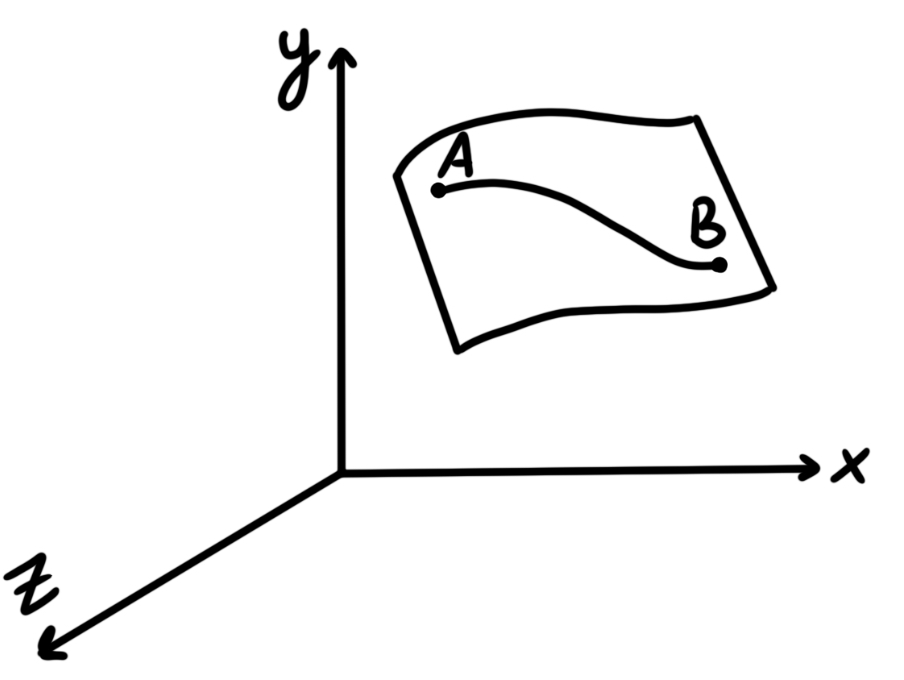
\includegraphics[width=0.3\textwidth]{/Users/vladbelousov/Desktop/Semestr_4-FP-NSU/АМ/Лекции_по_дням/image/4.png}
\end{center}


На этом рисунке мы выбрали \( \varphi_0  \) за ноль.

\begin{definition}[первый закон Кепелара]
    Планеты движутся по эллипсам в фокусе находится Солнце. 

    \[ \frac{ds}{dt }  = \frac{\frac{1}{2 } r (r d \varphi )}{dt } = \frac{M}{2 m }     -\text{секторальная скорость сохраняется }   \] 

\end{definition}

\begin{definition}[второй закон Кеплера]
    За равные промежутки времени радиус-вектор заметает одинаковые площади.
\end{definition}

Найдем связи между параметрами эллипсами и параметрами траектории: 

\[ r_{\min } = \frac{p}{1+e } ; \text{ } r_{\max } = \frac{p}{1-e}       \] 

\[ r_{\min } = DO ; \text{ } r_{\max } = OA     \]

\[ a =\frac{1}{2 }  ( r_{\max  } + r_{\min }  ) = \frac{p}{1- e ^2 } = \frac{\frac{M ^2 }{m \alpha } }{1- (1+ \frac{2M E }{m \alpha ^2 } )}= \frac{\alpha}{- 2E}  \Rightarrow a = \frac{\alpha}{2 |E|}   \] 

Расстояние от центра до оси: \( \displaystyle CO = \frac{1}{2 }  ( r_{\max  } - r_{\min  }  )= ae  \) 

\[ b = CB = a \sqrt{ 1 - e ^2 } \Rightarrow b = \frac{M}{\sqrt{2m|E|}}   \] 

\[  T =\frac{S_{\text{эл} } }{\dot{S} }= \frac{\pi ab }{\frac{M}{2m } } =\pi \alpha \sqrt{\frac{m}{2 |E| ^3} }     
\] 


\[ T^2 = 4 \pi ^2 \left( \frac{\alpha}{2 |E|}  \right) ^3 \Rightarrow T ^2 \sim a ^3 \Rightarrow   \] 

\begin{definition}[третий закон Кепелара]
    Квадраты периодов обращения планет вокруг Солнца относятся как кубы больших полуосей орбит планет.

    \[ \frac{T ^2 }{ a ^3 } = \mathrm{const}    \] 
\end{definition}

Задача Кеплера: 

\[ E = \mathrm{const}  \quad  \vec{ M }  = \overrightarrow{\mathrm{const}  } \quad k= 4, \text{ } S = 3  \] 

S = 3 - степени свободы, это минимальное количество параметров, необходимых для описания системы.

k - число интегралов движения, если S = k - задача называется полностью интегрируема.

S>k - задача супер интегрируема

\[ \vec{n }  = \frac{ \vec{r } }{r } \quad  dn = n d \varphi \Rightarrow \frac{dn}{dt }   = \dot{ \varphi}    \] 

\begin{center}
    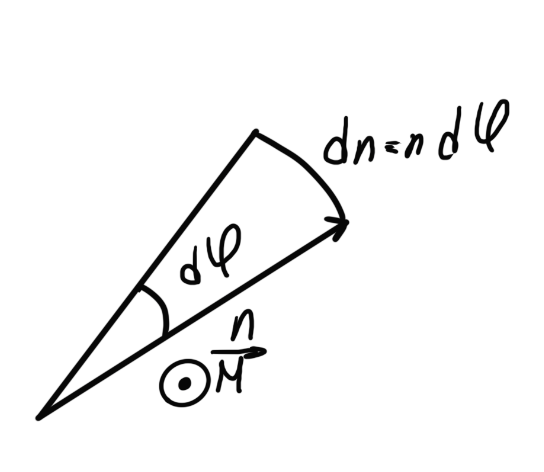
\includegraphics[width=0.2\textwidth]{/Users/vladbelousov/Desktop/Semestr_4-FP-NSU/АМ/Лекции_по_дням/image/5.png}
\end{center}

\[ d \vec{n }  \parallel \vec{M }  \times  \vec{ n}   \] 

\[ \frac{d \vec{n }  }{rt}= \frac{\vec{M } }{m r ^2 } \times  \vec{n }  \overset{(1)}{=} - \frac{ \vec{M } }{\alpha } \times  \frac{d \vec{v } }{dt }    \Rightarrow \frac{d}{dt } \underbrace{\left(  \vec{v } \times \vec{M }    - \alpha \frac{ \vec{r } }{r}   \right)}_{\vec{A} } =0 \quad \bigg | \vec{ n }= \vec{e_r}      \] 

\[ \vec{F }  = \frac{m d \vec{v } }{ dt }    = - \frac{\alpha}{r ^2 }m  \quad (1) \] 

Где \( \vec{A }  \)  - это вектор Лапласа-Рунге-Ленца

\[ \vec{A }  \cdot   \vec{r }  = A r \cos \xi \] 

Подставим чему равно \( \vec{A }  \) 

\[ \vec{r } [\vec{v } \times  \vec{M } ]  - \alpha \frac{ \vec{r }  \vec{r } }{r }  = \vec{M }  [\vec{r} \times \vec{ v}    ]- \alpha r = \vec{M }  \frac{ \vec{M } }{m}- \alpha r = A r \cos \xi    \] 

\[ r(\alpha + A \cos \xi   ) = \frac{M ^2 }{m}  \Rightarrow r = \frac{ \frac{ M ^2 }{m \alpha } }{1+ \underbrace{\frac{A}{2 }}_{=e}  \cos \xi }  \] 
 
Закон сохранения \( \displaystyle  \frac{d}{dt } \vec{A }  =0  \) получается из симметрии 4-ч мерного пространства.

\section{Задача рассеяния }

\begin{center}
    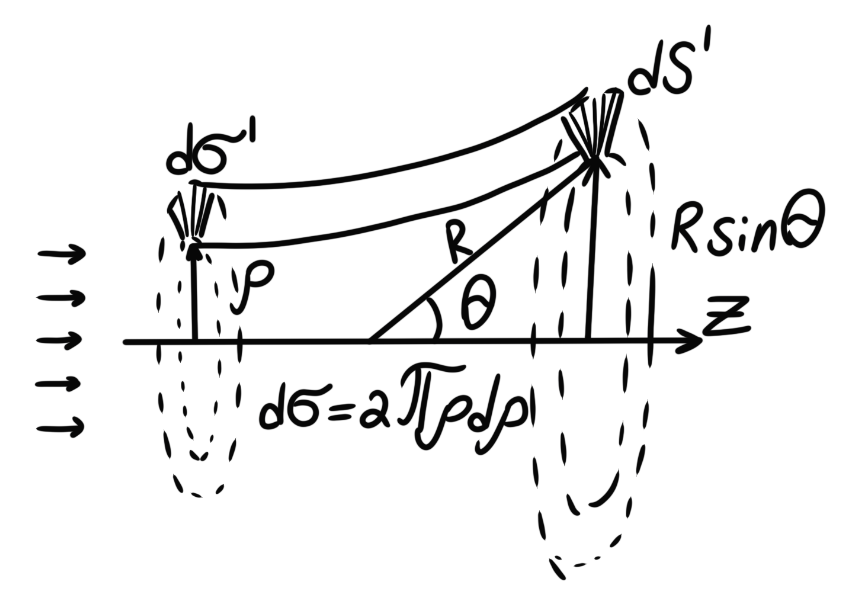
\includegraphics[width=0.5\textwidth]{/Users/vladbelousov/Desktop/Semestr_4-FP-NSU/АМ/Лекции_по_дням/image/6.png}
\end{center}

\[ \rho - \text{ прицельный параметр} ; \quad  \theta - \text{угол рассеяния}   \] 

\[ dS = 2 \pi R \sin  \theta R d \theta \] 

\[ \frac{d \sigma'}{d \sigma} = \frac{d S ' }{ dS }   \] 

\[ d \sigma ' = d \sigma \frac{dS'}{2 \pi R \sin \theta R d \theta  } = d \sigma \frac{d \Omega}{2 \pi \sin \theta d \theta }  \] 

\[ \frac{d \sigma ' }{ d \Omega '} = \frac{d \sigma }{2 \pi \sin \theta d \theta}  \] 

\[ d\dot{N } = d \sigma ' I \underbrace{S_n}_{-\text{поток } } k=d \sigma ' \frac{d \Omega' }{d \Omega ' }I k S_n \Rightarrow \frac{d \sigma '}{d \Omega '} = \frac{d\dot{N} }{Ik S_n d \Omega'}  -\text{экспериментальная формула}   \] 

\[ \frac{d \sigma ' }{d \Omega ' } = \frac{2 \pi \rho d \varphi }{2 \pi \sin \theta d \theta } = \frac{\rho (\theta )}{\sin \theta } \left\lvert \frac{d \rho }{d \theta }  \right\rvert   \] 

\begin{center}
    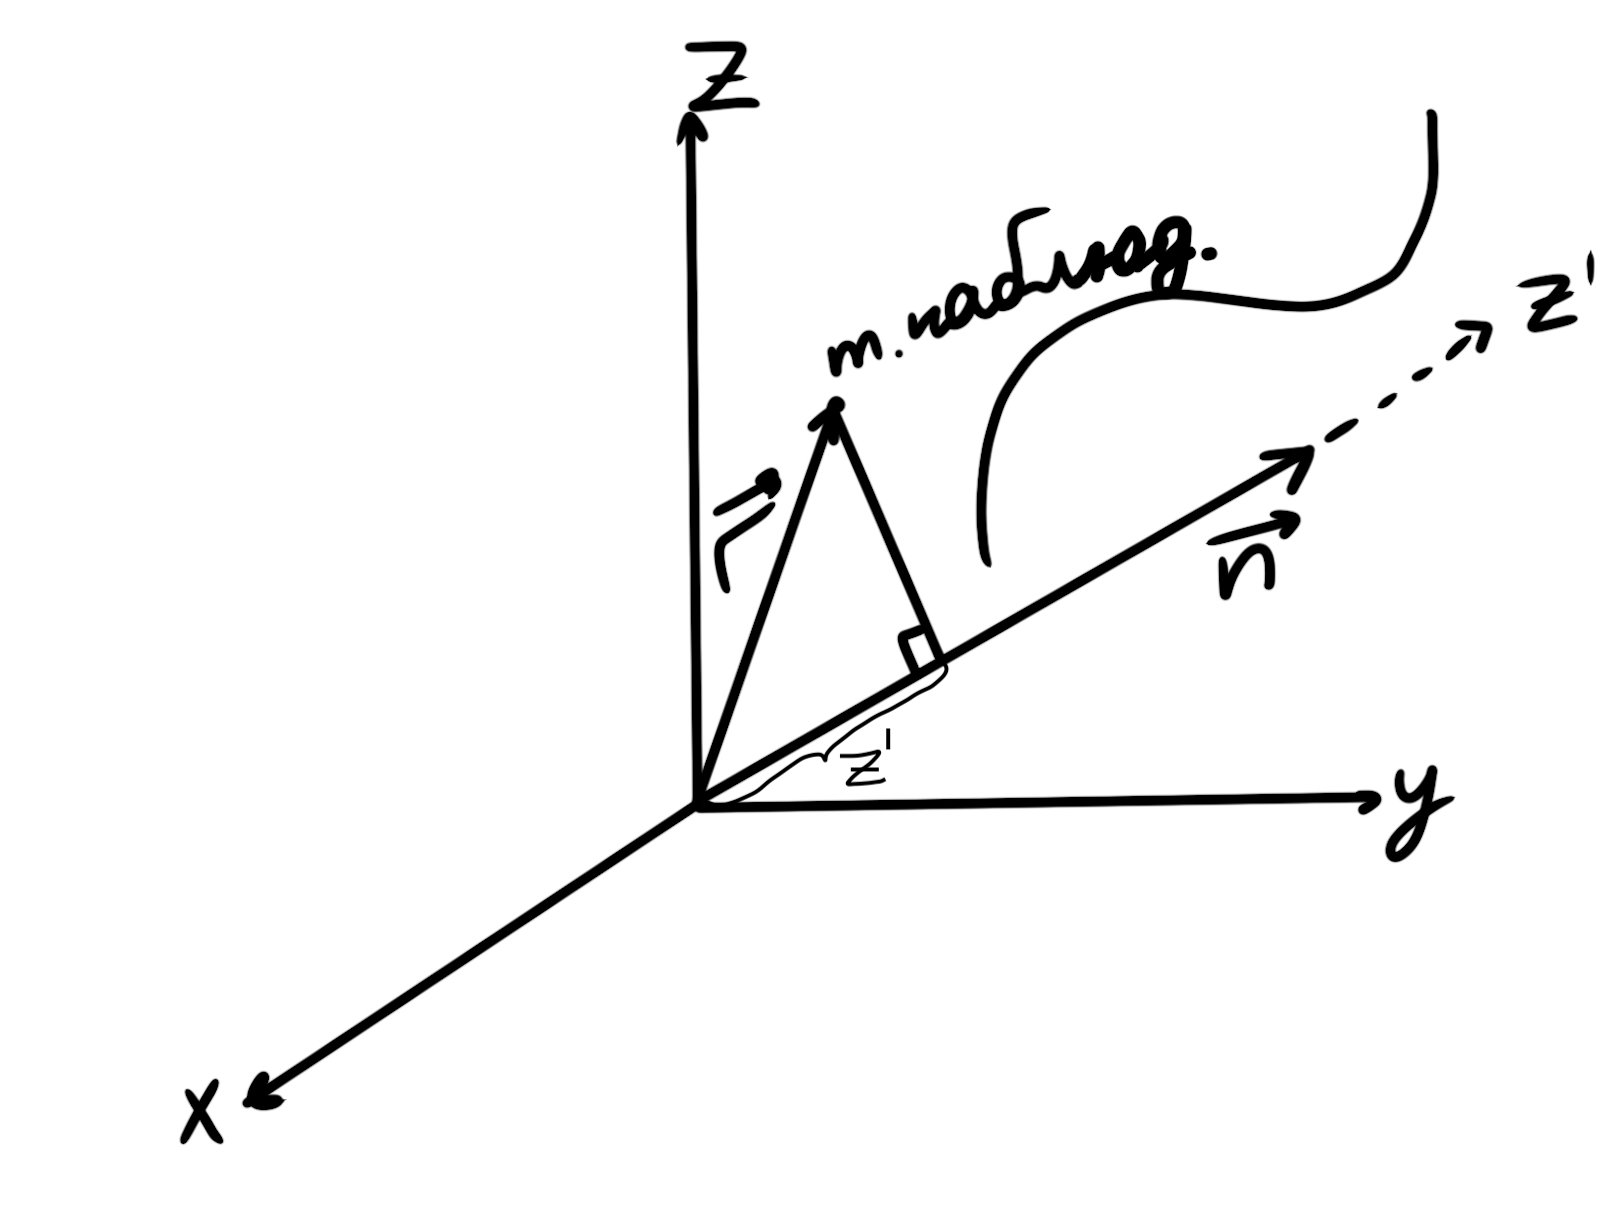
\includegraphics[width=0.4\textwidth]{/Users/vladbelousov/Desktop/Semestr_4-FP-NSU/АМ/Лекции_по_дням/image/7.png}
\end{center}

\[ \int_{0}^{\varphi_0 }d \varphi = \int_{r=\infty }^{r_0 } \frac{ \frac{ M }{mr ^2 } }{\sqrt{\frac{2}{m } \left( E  - \frac{\alpha}{r }  - \frac{M ^2 }{2 m r ^2 }  \right)}}    \] 

\[ \rho( \theta ) = \frac{\alpha}{2 E }  ctg \frac{\theta}{2}  \] 

\[ r= \frac{ p }{-1 +e \cos (\varphi- \varphi_0 )}  \] 

\[   \frac{d \sigma }{d \Omega } = \left(  \frac{\alpha}{ 4 E }    \right) ^2 \frac{1}{\sin ^2  \frac{\theta}{2} }  - \text{формула Резерфорда}  \] 

\begin{center}
    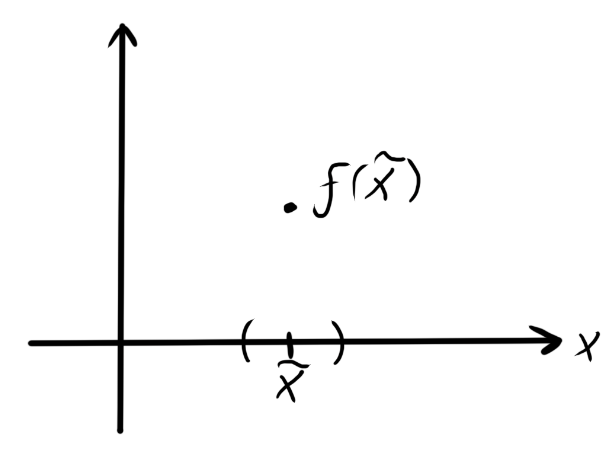
\includegraphics[width=0.5\textwidth]{/Users/vladbelousov/Desktop/Semestr_4-FP-NSU/АМ/Лекции_по_дням/image/8.png}
\end{center}

a) \( E \gg U_{\text{хар}}    \) 

b) \( \rho \ll a_{\text{хар}}   \) 

\[ \sin  \gamma = \frac{\rho}{r }    \] 

\[ P_x = P_x' = m v_{\infty }  \] 

\[ F_y= - \frac{\partial  U }{\partial  r }\sin  \gamma= - \frac{\partial  U }{\partial  r } \frac{\rho}{r}    \] 

\[ F_y= \frac{d P_y ' }{dt}  \] 

\[ P_y' = \int_{-\infty}^{\infty} F_y dt = - \int_{-\infty}^{\infty} \frac{\partial  U }{\partial  r } \frac{\rho}{r } \frac{dt}{v_{\infty  } } v_{\infty } \boxed{= }     \] 

\[ x= t v_{\infty  } \quad  x= \sqrt{r ^2 - \rho ^2 } \Rightarrow dx = \frac{r dt }{\sqrt{r ^2 - \rho ^2 }}   \] 

\[ \boxed{= } - \frac{\rho}{v_{\infty  } } \int_{-\infty}^{\infty} \frac{d U }{dr } \frac{dr}{r } = -2 \frac{\rho}{v_{\infty  } }\int_{-\infty}^{\infty} \frac{dU}{dr }     \frac{dr}{\sqrt{r ^2 - \rho ^2 } } = P_y'     \] 

\[ tg \theta \approx \theta = \frac{P_y ' }{ P_x ' } \Rightarrow  \underbrace{\boxed{\theta \approx - \frac{2 \rho }{m v_{\infty  } ^2 } \int _{-\infty}^{\infty} \frac{d U }{dr } \frac{dr}{\sqrt{r ^2 - \rho ^2 } }  } }_{\displaystyle \Rightarrow \rho(\theta) }   \] 

%%-------------------------------%%

% Закрытие документа, если файл компилируется отдельно
\ifdefined\mainfile
    % Если это основной файл, не нужно заканчивать документ
\else
    \end{document}
\fi